\documentclass{beamer}

%lembre-se de configurar o pdflatex com:
%pdflatex -shell-escape -synctex=1 -interaction=nonstopmode  -output-directory=build  %.tex

\usepackage{aula}

\title{Introdução a Algoritmos}
\date{\today}

\begin{document}
    
\input{capa}

\begin{frame}{Metodologias Ágeis — Conceito}
    
    Metodologias ágeis são formas de organizar o desenvolvimento de software de maneira:
    
    \begin{itemize}
        \item Iterativa (em pequenos passos)
        \item Flexível (adaptável a mudanças)
        \item Colaborativa (equipe + usuário)
    \end{itemize}
    
    \vspace{0.4cm}
    
    \textbf{Ideia principal:}
    
    \begin{itemize}
        \item Entregar valor rapidamente
        \item Melhorar continuamente
    \end{itemize}
    
    \vspace{0.4cm}
    
    Exemplos:
    
    \begin{itemize}
        \item Scrum
        \item Kanban
    \end{itemize}
    
\end{frame}

\begin{frame}{User Stories — O que são?}
    
    User Stories descrevem funcionalidades do ponto de vista do usuário.
    
    \vspace{0.4cm}
    
    Formato clássico:
    
    \begin{block}{User Story}
        Como \textbf{[tipo de usuário]} \\
        Quero \textbf{[objetivo]} \\
        Para \textbf{[benefício]}
    \end{block}
    
    \vspace{0.4cm}
    
    Exemplo:
    
    \begin{block}{Exemplo}
        Como \textbf{analista GIS} \\
        Quero \textbf{carregar um shapefile} \\
        Para \textbf{visualizar dados no mapa}
    \end{block}
    
\end{frame}

\begin{frame}{User Stories — Boas práticas}
    
    Boas user stories devem ser:
    
    \begin{itemize}
        \item \textbf{Simples} e fáceis de entender
        \item \textbf{Pequenas} (podem ser implementadas rapidamente)
        \item \textbf{Focadas no usuário}
    \end{itemize}
    
    \vspace{0.4cm}
    
    \textbf{Evitar:}
    
    \begin{itemize}
        \item Detalhes técnicos excessivos
        \item Histórias muito grandes
    \end{itemize}
    
    \vspace{0.4cm}
    
    \textbf{Dica:}
    
    Se está muito grande → dividir em várias histórias.
    
\end{frame}

\begin{frame}{Kanban — Organização do trabalho}
    
    Kanban é um método visual para acompanhar tarefas.
    
    \vspace{0.4cm}
    
    \begin{center}
        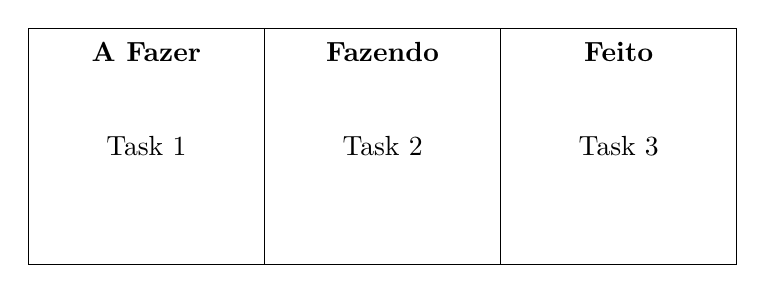
\begin{tikzpicture}
            
            \draw (0,0) rectangle (9,3);
            
            \draw (3,0) -- (3,3);
            \draw (6,0) -- (6,3);
            
            \node at (1.5,2.7) {\textbf{A Fazer}};
            \node at (4.5,2.7) {\textbf{Fazendo}};
            \node at (7.5,2.7) {\textbf{Feito}};
            
            \node at (1.5,1.5) {Task 1};
            \node at (4.5,1.5) {Task 2};
            \node at (7.5,1.5) {Task 3};
            
        \end{tikzpicture}
    \end{center}
    
    \vspace{0.3cm}
    
    \begin{itemize}
        \item Cada tarefa é um cartão
        \item Cartões se movem entre colunas
    \end{itemize}
    
\end{frame}

\begin{frame}{User Stories + Kanban}
    
    Como usar juntos:
    
    \vspace{0.3cm}
    
    \begin{itemize}
        \item User stories definem \textbf{o que fazer}
        \item Kanban organiza \textbf{o andamento}
    \end{itemize}
    
    \vspace{0.4cm}
    
    Fluxo típico:
    
    \begin{enumerate}
        \item Escrever user stories
        \item Colocar no quadro Kanban
        \item Implementar uma por vez
        \item Mover para "Feito"
    \end{enumerate}
    
    \vspace{0.4cm}
    
    \textbf{Benefícios:}
    
    \begin{itemize}
        \item Organização visual
        \item Foco no usuário
        \item Entregas contínuas
    \end{itemize}
    
\end{frame}

\end{document}
